The unit card shows the current capabilities of a trooper in power armor and tracks damage.
A unit card can be formatted in any way so long as it contains all the essential information.
Below is a sample unit card for a power armor trooper.

\begin{figure}[!h]
  \centering
  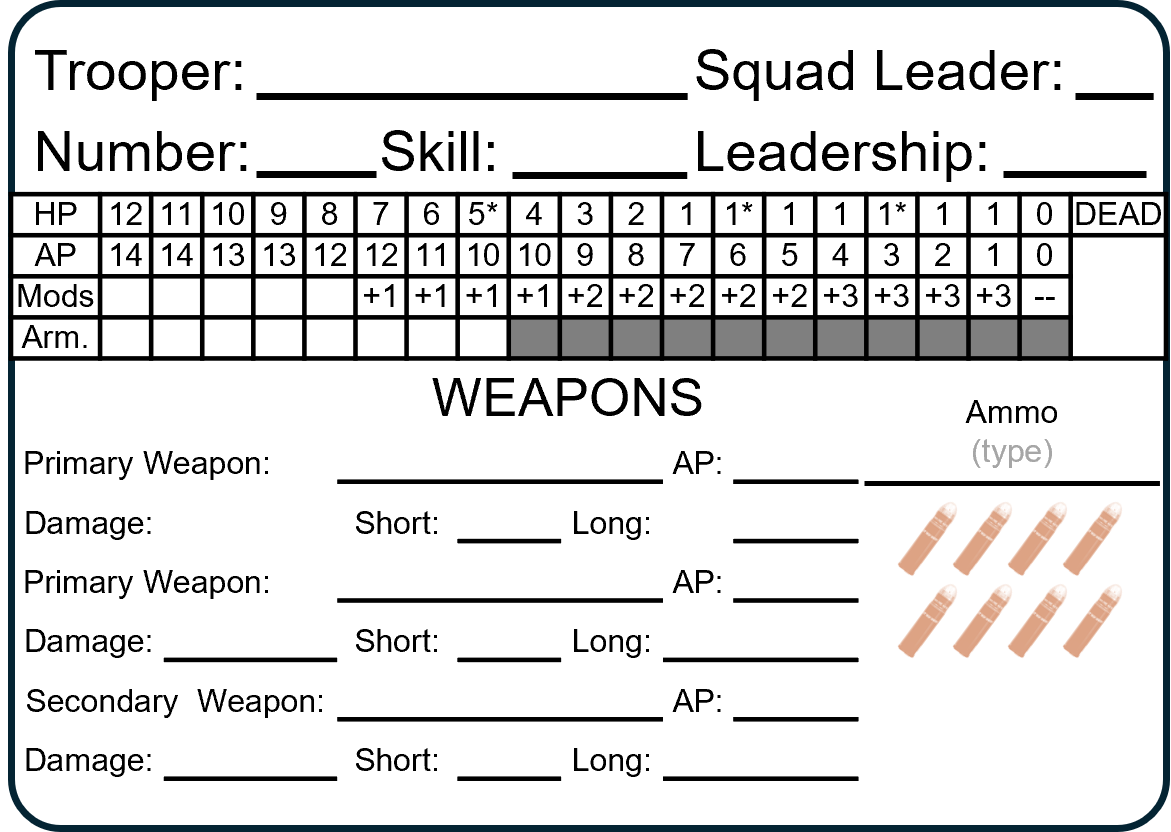
\includegraphics[alt='Sample Power Armor Trooper', width=5.63in, height=4in]{img/PowerArmorTrooper.png}
  \caption*{Power Armor Trooper Unit Card}
\end{figure}

There are a few key differences between the standard trooper unit card and a power armor trooper unit card.

Standard power armor has 6 cells of armor.
Basic power armor has only 4 cells of armor and heavy power armor has 8 cells of armor.
All other cells of armor should be marked off before the game.

Power armor troopers ignore bludgeoning damage (\textbackslash).
However, 9 or more points of bludgeoning damage in a single turn will knock a power armor trooper prone.
Standard damage (X) destroys armor before damaging HP cells.
If a single attack does more damage than the remaining armor, first mark all remaining armor and then mark HP cells starting with the 12 HP cell.

Once all of the armor has been destroyed, then the trooper's HP cells are marked.
Power armor protects the trooper, giving them more HP than a basic trooper.
HP cells are fully crossed out when the trooper takes standard damage (X).
The current HP of the trooper is given by the first cell to the right of the highest fully marked HP cell.
For example, if the trooper has HP 10, 9, and 6 marked off, their current HP is 5.
When marking damage, you still roll 2D6 and apply damage starting with the first unmarked HP cell to the right of the rolled value.

The HP cells marked with * indicate significant damage to the power armor.
When one of these cells is fully marked, the opponent may choose one of the weapon systems to disable on the power armor suit.
When two of these cells have been fully marked, the jet pack on the suit no longer functions.

Total action points (AP) for the trooper are given in the AP section.
Power armor greatly extends the capabilities of troopers, giving them more AP.
Use the value in the column corresponding to the trooper's current HP.
For example, if the trooper has 5 HP, then they have only 10 AP.

As with standard troopers, green troopers in power armor reduce all of their AP values by 1, while veteran troopers increase all values by 1 and elite troopers increase all values by 2.

Similarly, the modifier section tracks the current modifier for the trooper's target numbers based upon current HP.
For example, if the trooper has 5 HP, then add +1 to all target numbers.

Basic and standard power armor comes equipped with a jet pack.
Heavy power armor is too bulky to use a jet pack.

The weapons and equipment section list the primary and secondary weapons the trooper is equipped with, along with their damage values and range brackets.
Power armor troopers cannot use grenades but may use satchel changes.

The leadership section lists the squad leader for the trooper and their leadership score.
This section contains the information required for morale checks.
